\chapter{Introduction}
\begingroup
\justifying
\setlength{\parindent}{0pt}
\setstretch{2}
\setlength{\parskip}{0.5\baselineskip}
\titlespacing{\chapter}{0pt}{0pt}{0pt}
\titlespacing{\section}{0pt}{0pt}{0pt}

This chapter \lipsum[1]

\section{Motivations}

This thesis deals with the problem of the blind multiuser detection for DS-CDMA. This thesis deals with the problem of the blind multiuser detection for DS-CDMA...

\begin{equation}
J_{4\times 6} = \left[\dot{p}^{(1)},\, \dot{p}^{(2)},\, \dots,\, \dot{p}^{(6)}\right]
\end{equation}

\lipsum[1-2]

\section{Objectives and Scope}

The communication channel considered in this thesis is assumed to be slow time-varying. \lipsum[1]

Wireless communication is evolving rapidly \cite{jordan2002,padgett1995}.

\section{Organisation}

\lipsum[1-2]

\begin{figure}[h]
    \centering
    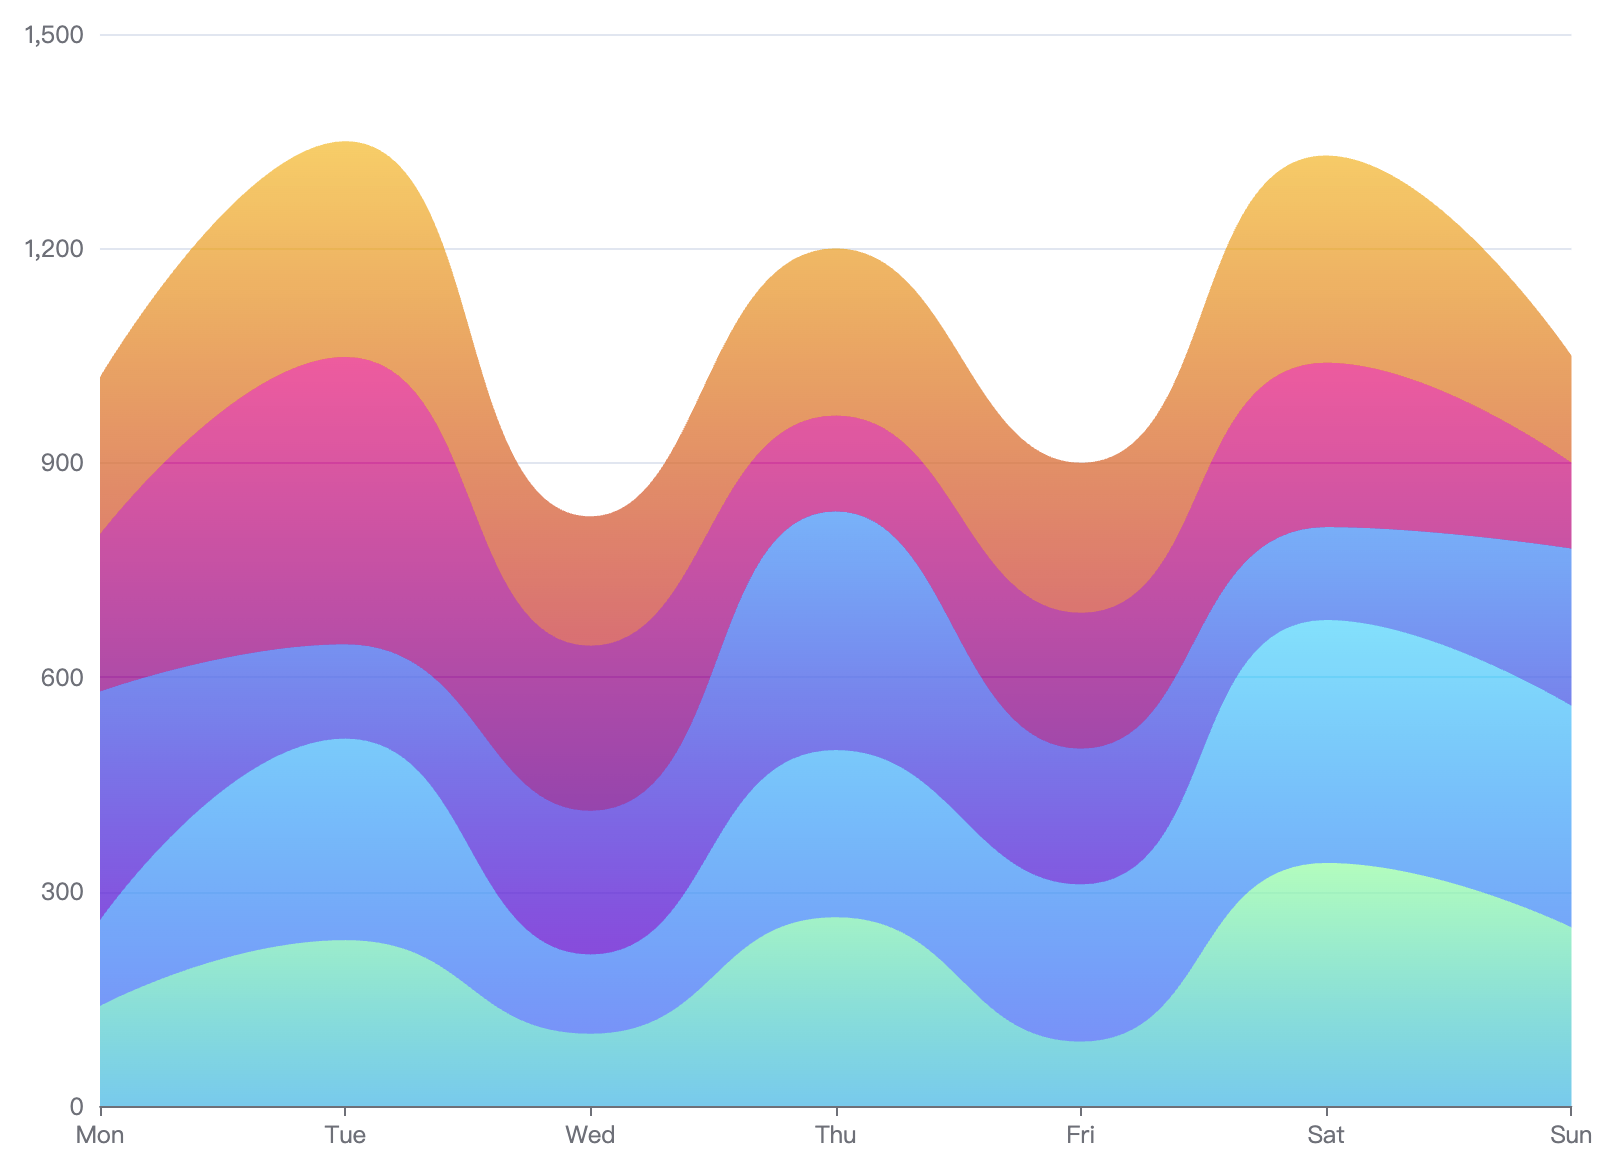
\includegraphics[width=0.6\textwidth]{assets/figures/demo.png}
    \caption{Proposed CMCN architecture}
    \label{fig:cmcn}
\end{figure}

\endgroup